\documentclass[10pt]{beamer}

\input{/Users/daniel/Documents/LaTeX/beamer-style.tex}


\title{Développement d'applications mobiles}
\subtitle{Chapitre 1 : Installation}
\date{\today}
\author{Daniel Schreurs}
\institute{Haute École de la Province de Liège}
%\titlegraphic{\hfill\includegraphics[height=1.5cm]{logo.eps}}

\begin{document}

\maketitle

\setbeamerfont{subsection in toc}{size=\small}
\begin{frame}[allowframebreaks]{Table des matières}
    \setbeamertemplate{section in toc}[sections numbered]
    \tableofcontents
\end{frame}

\section{Installation}

\subsection{Liste des logiciels à installer}
\begin{frame}[fragile,t]{\secname : \subsecname}
    \begin{itemize}
        \item \href{https://git-scm.com/downloads}{git} (si ce n'est déjà fait);
        \item \href{https://flutter.dev/docs/get-started/install}{Flutter SDK 3.*.*} ;
        \item \href{https://dart.dev/get-dart}{Dart SDK};
        \item \href{https://itunes.apple.com/us/app/xcode/id497799835}{Xcode} (si vous êtes sous macOS);
        \item \href{https://guides.cocoapods.org/using/getting-started.html#installation}{Cocoapods} (si vous êtes sous macOS);
        \item \href{https://www.jetbrains.com/fr-fr/idea/download/#section=mac}{IntelliJ IDEA} avec les plugins:
              \begin{itemize}
                  \item \href{https://plugins.jetbrains.com/plugin/9212-flutter}{Flutter} ;
                  \item \href{https://plugins.jetbrains.com/plugin/16602-embedded-dartpad}{Dartpad} (pour tester des exemples Dart).
              \end{itemize}
    \end{itemize}
\end{frame}

\subsection{Guide d'installation}
\begin{frame}[fragile,t]{\secname : \subsecname}
    \begin{center}
        \href{https://flutter.dev/docs/get-started/install}{GET STARTED !}
    \end{center}
    À l'issue du processus d'installation, vous devez depuis votre terminal être capable d’exécuter cette commande :
    \begin{lstlisting}[caption={Connaître la version de flutter},language=C, label=getversion]
    flutter --version
    \end{lstlisting}
\end{frame}

\subsection{Flutter Doctor}
\begin{frame}[fragile,t]{\secname : \subsecname}
    L’analyse de la commande \textit{flutter doctor} révèle plusieurs choses :
    \begin{itemize}
        \item Elle vérifie la version de Flutter actuellement installée;
        \item Elle vérifie la licence Android;
        \item Elle détecte la présence d’IntelliJ IDEA\footnote{Et a vérifié la présence des plug-ins de Flutter  et Dart.};
        \item Elle détecte la présence d'un périphérique ou simulateur.
    \end{itemize}
    \begin{lstlisting}[caption={Vérifier l'installation},language=bash, label=getversion]
        flutter doctor
        \end{lstlisting}
\end{frame}
\begin{frame}[fragile,t]{\secname : \subsecname}
    \begin{figure}[H]
        \begin{center}
            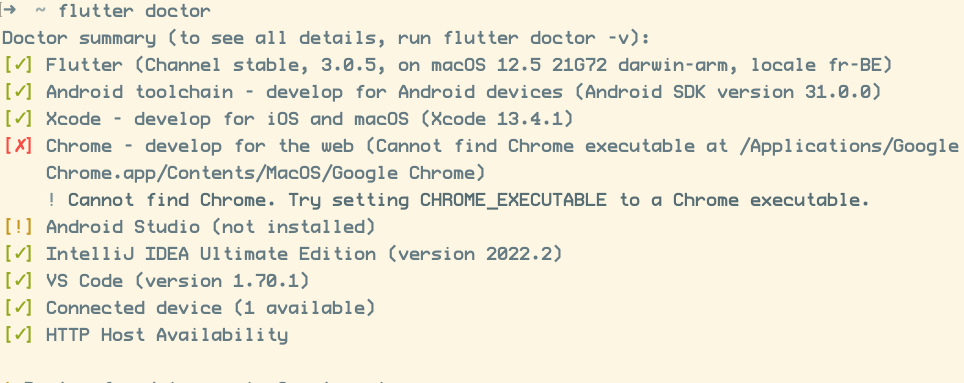
\includegraphics[width=\textwidth]{../assets/img/flutter-doctor.jpg}
            \caption*{flutter doctor}
        \end{center}
    \end{figure}
\end{frame}


\section{Première application}
\subsection{Création d'un nouveau projet}
\begin{frame}[fragile,t]{\secname : \subsecname}
    \begin{figure}[H]
        \begin{center}
            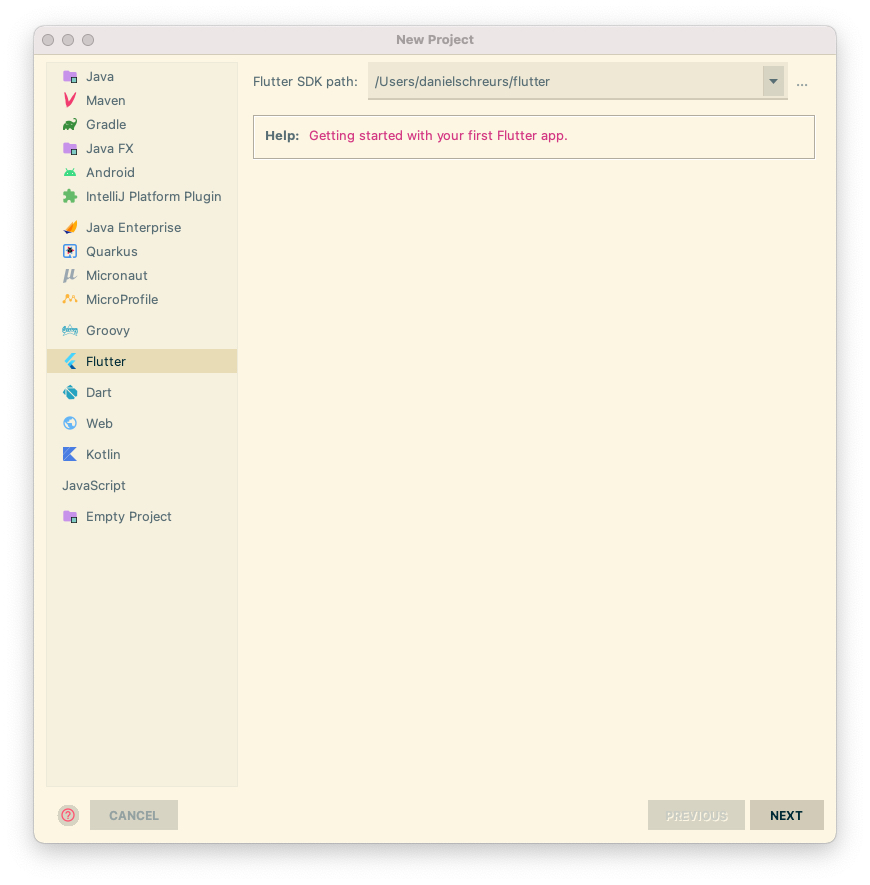
\includegraphics[width=0.4\textwidth]{../assets/img/new-project-1.jpg}
            \caption*{Création d'un nouveau projet Flutter depuis IntelliJ IDEA}
            \label{Fig:new-project-1}
        \end{center}
    \end{figure}
\end{frame}


\subsection{Configurer un nouveau projet}
\begin{frame}[fragile,t]{\secname : \subsecname}
    \begin{columns}
        \column{0.7\textwidth}
        \begin{figure}[H]
            \begin{center}
                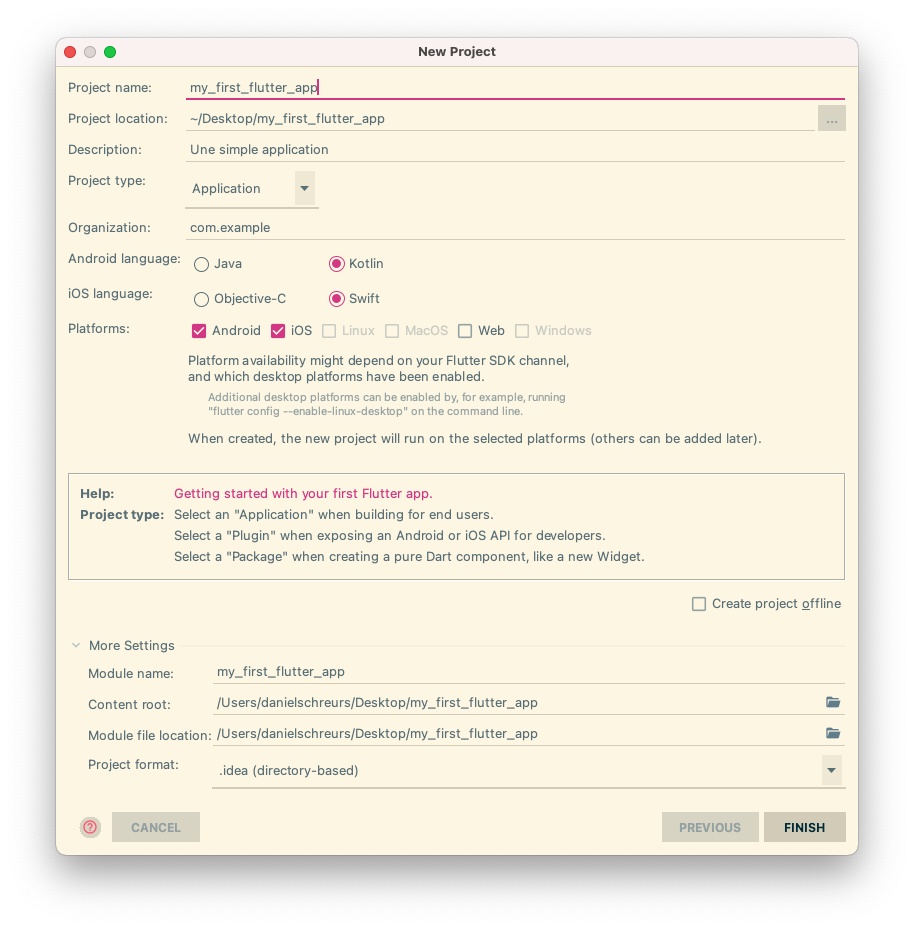
\includegraphics[width=0.6\textwidth]{../assets/img/new-project-2.jpg}
                \caption*{Configuration du nouveau projet Flutter depuis IntelliJ IDEA}
                \label{Fig:new-project-2}
            \end{center}
        \end{figure}
        \column{0.3\textwidth}
        \metroset{block=fill}
        \begin{block}{Remarque}
            Attention au $nom\_du\_projet$. Il faut suivre la convention $[a-z0-9\_]$ (\href{https://dart.dev/tools/pub/pubspec#name}{Documentation})
        \end{block}
    \end{columns}
\end{frame}

\subsection{Choisir un périphérique}
\begin{frame}[fragile,t]{\secname : \subsecname}
    \begin{figure}[H]
        \begin{center}
            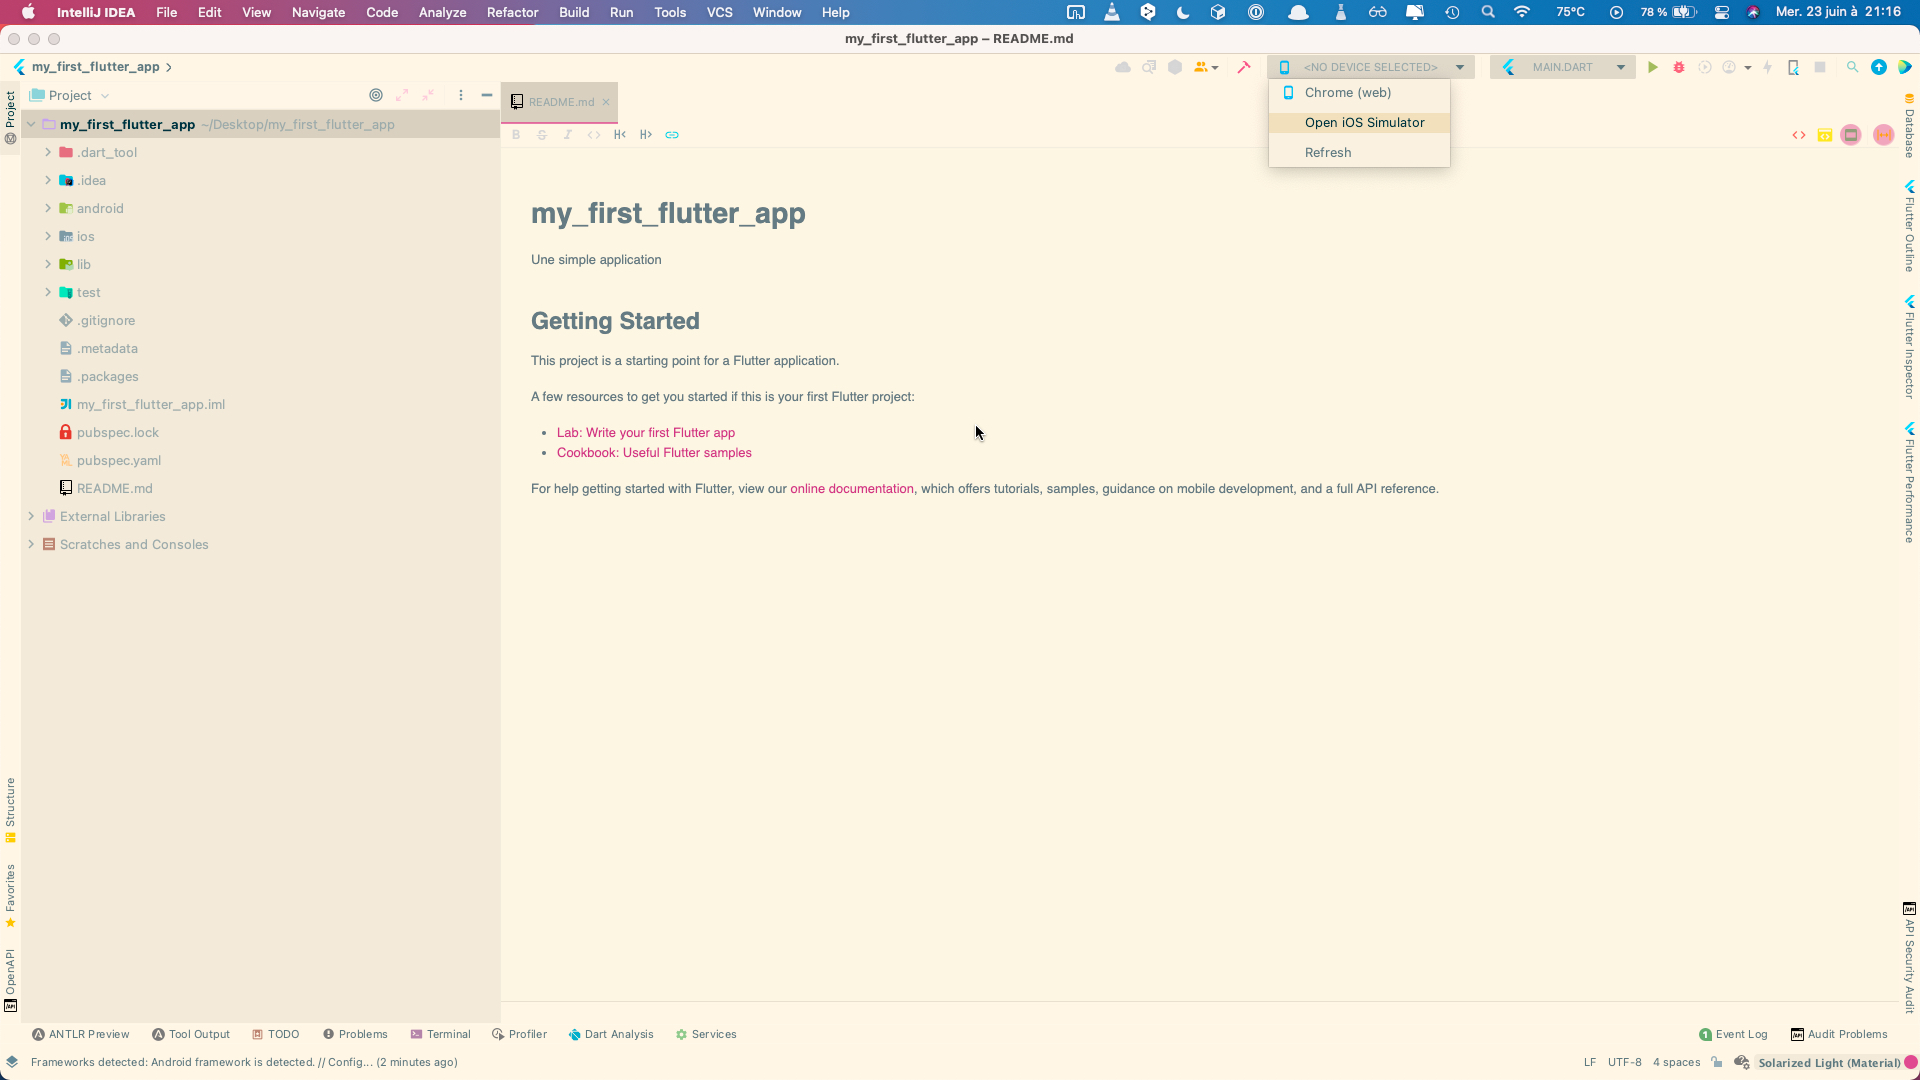
\includegraphics[width=0.85\textwidth]{../assets/img/new-project-3.jpg}
            \caption*{Demander à ouvrir un simulateur}
            \label{Fig:new-project-3}
        \end{center}
    \end{figure}
\end{frame}

\subsection{Lancer l'application}
\begin{frame}[fragile,t]{\secname : \subsecname}
    \begin{figure}[H]
        \begin{center}
            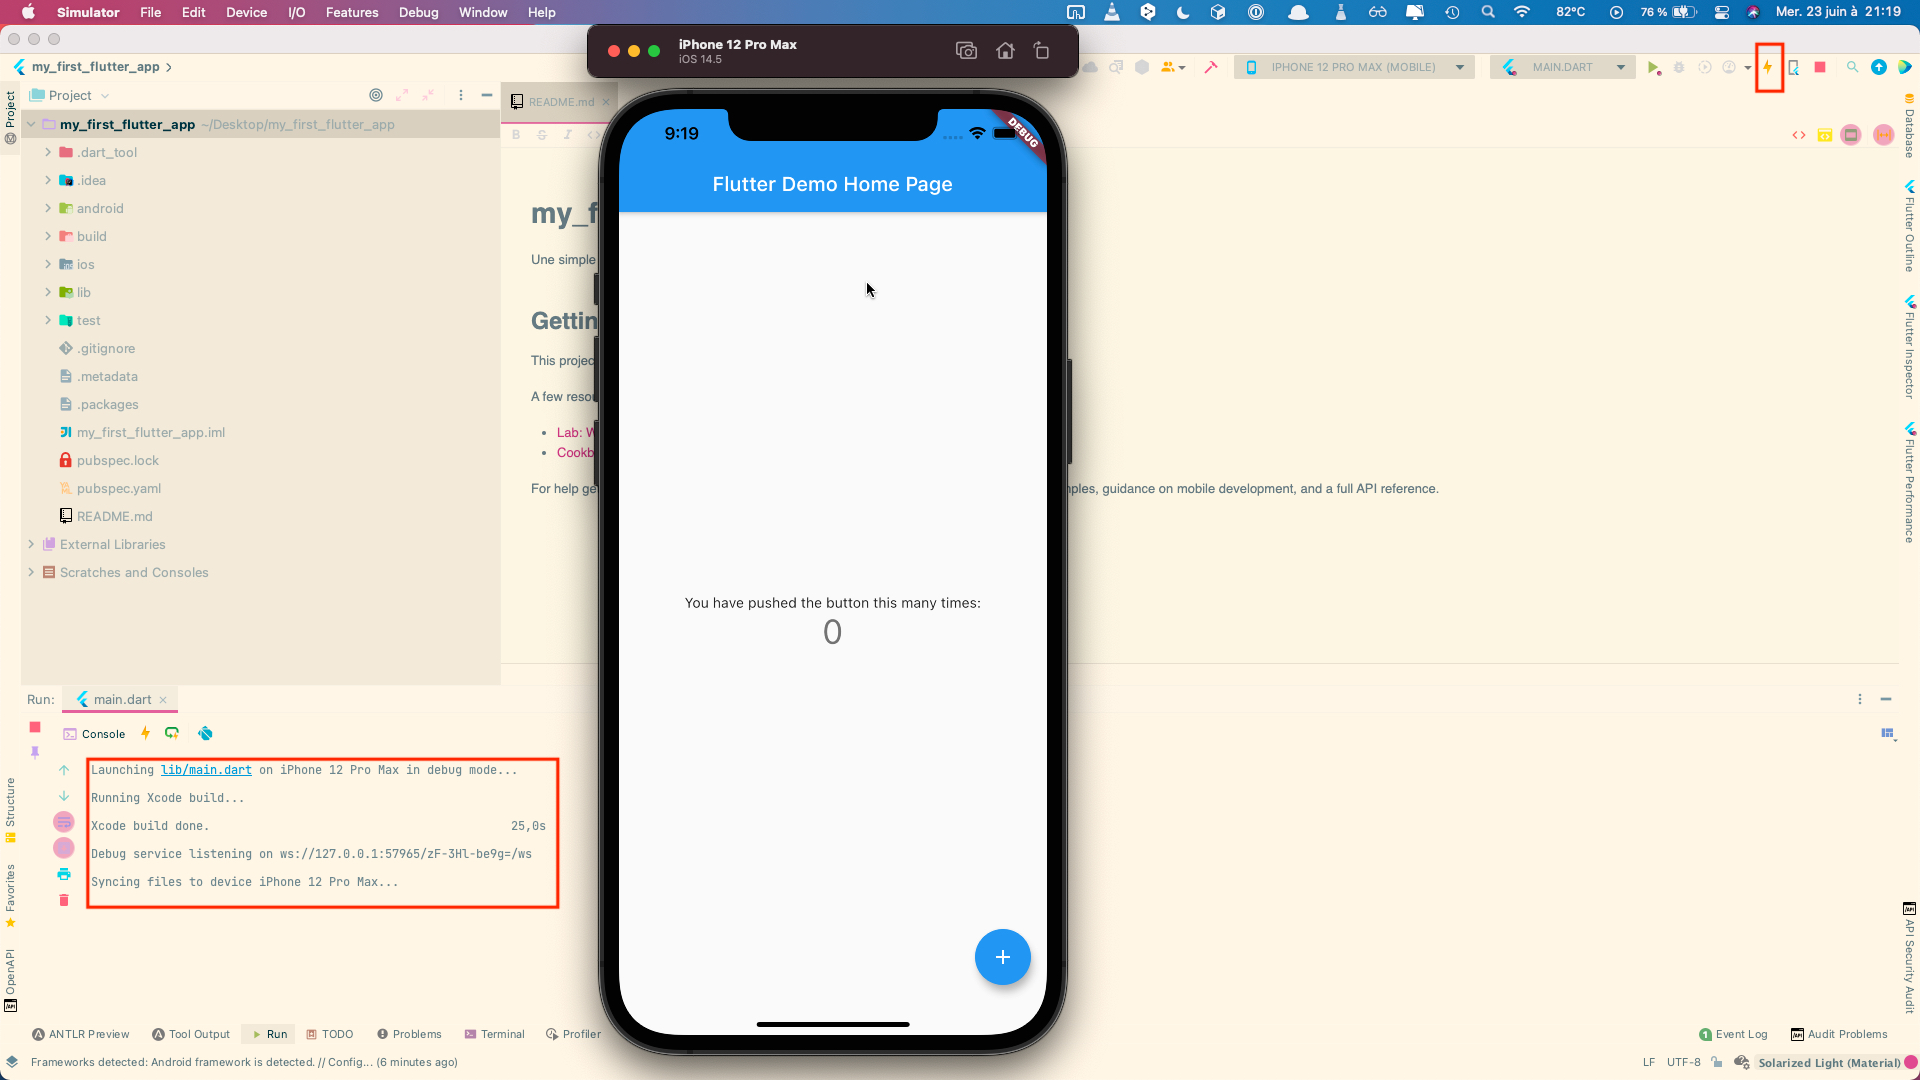
\includegraphics[width=0.85\textwidth]{../assets/img/new-project-5.jpg}
            \caption*{Démarrer l'application dans le simulateur}
            \label{Fig:new-project-5}
        \end{center}
    \end{figure}
\end{frame}

\subsection{En cas de problème}
\begin{frame}[fragile,t]{\secname : \subsecname}
    \begin{itemize}
        \item La documentation de Flutter : \href{flutter.dev}{flutter.dev}
        \item La documentation de Dart : \href{dart.dev}{dart.dev}
        \item Les autres : \href{https://flutter.dev/community}{flutter.dev/community}
        \item La chaine officielle sur YouTube : \href{https://www.youtube.com/c/flutterdev/}{youtube.com/c/flutterdev}
    \end{itemize}
\end{frame}

\end{document}